\chapter{History of speakers}
%The history of the language family’s speakers starting from some point in history that will eventually lead in not that much detail to the change in the education system that was a significant contribution to the decrease in the speaker population. This leads to the more recent historical and also current situation of what languages are spoken where in the region, how transportation changes have affected their interactions, etc., which leads into the 
%\subsection{History}
\label{chap:Tipije}
\largerpage
Knowing the history of the speech community helps to understand the length and intensity of exposure to today's contact languages, and to identify possible past dwelling places of speakers. The exact history of Vamale speakers is poorly studied. This section mainly aims at reconstructing the approximate distribution and the contact languages prior to the major population movements of 1904 and 1917, and to give a brief overview of the reasons why the language lost so many speakers.
The account given here is different from the situation described in detail by \textcite[91--93]{guiart_donnees_1984}, and yet different from \textcite[20]{leenhardt_evenements_1978a}, partly because most clans have changed names. The following is a summary of written and oral sources; some details remain unclear.

\section{Pre-1917}
Pamare (the Paicî name)/Pamale/Vamale is the name of a river tributary to the Tipije, flowing northwards from (Na Unu) Pamale mountain, just southwest of the Cigu \~ Tchingou massif. Oriented almost exactly south-north, it flows from an area today uninhabited and bordered by Cèmuhî speakers (see \figref{map:pamale}), until it unites with the Vawe river,\footnote{The Vawe tribe is mentioned in \textcite[26]{leenhardt_figures_1978} as well as in \textcite{sand_tiouande_2001}, and the Pei and Fouan clans claim to be from there.} at a river bend and becomes the Tipije \~ Tipindjé river, joined after a few kilometres by the Usa creek. 

\begin{figure}
% 	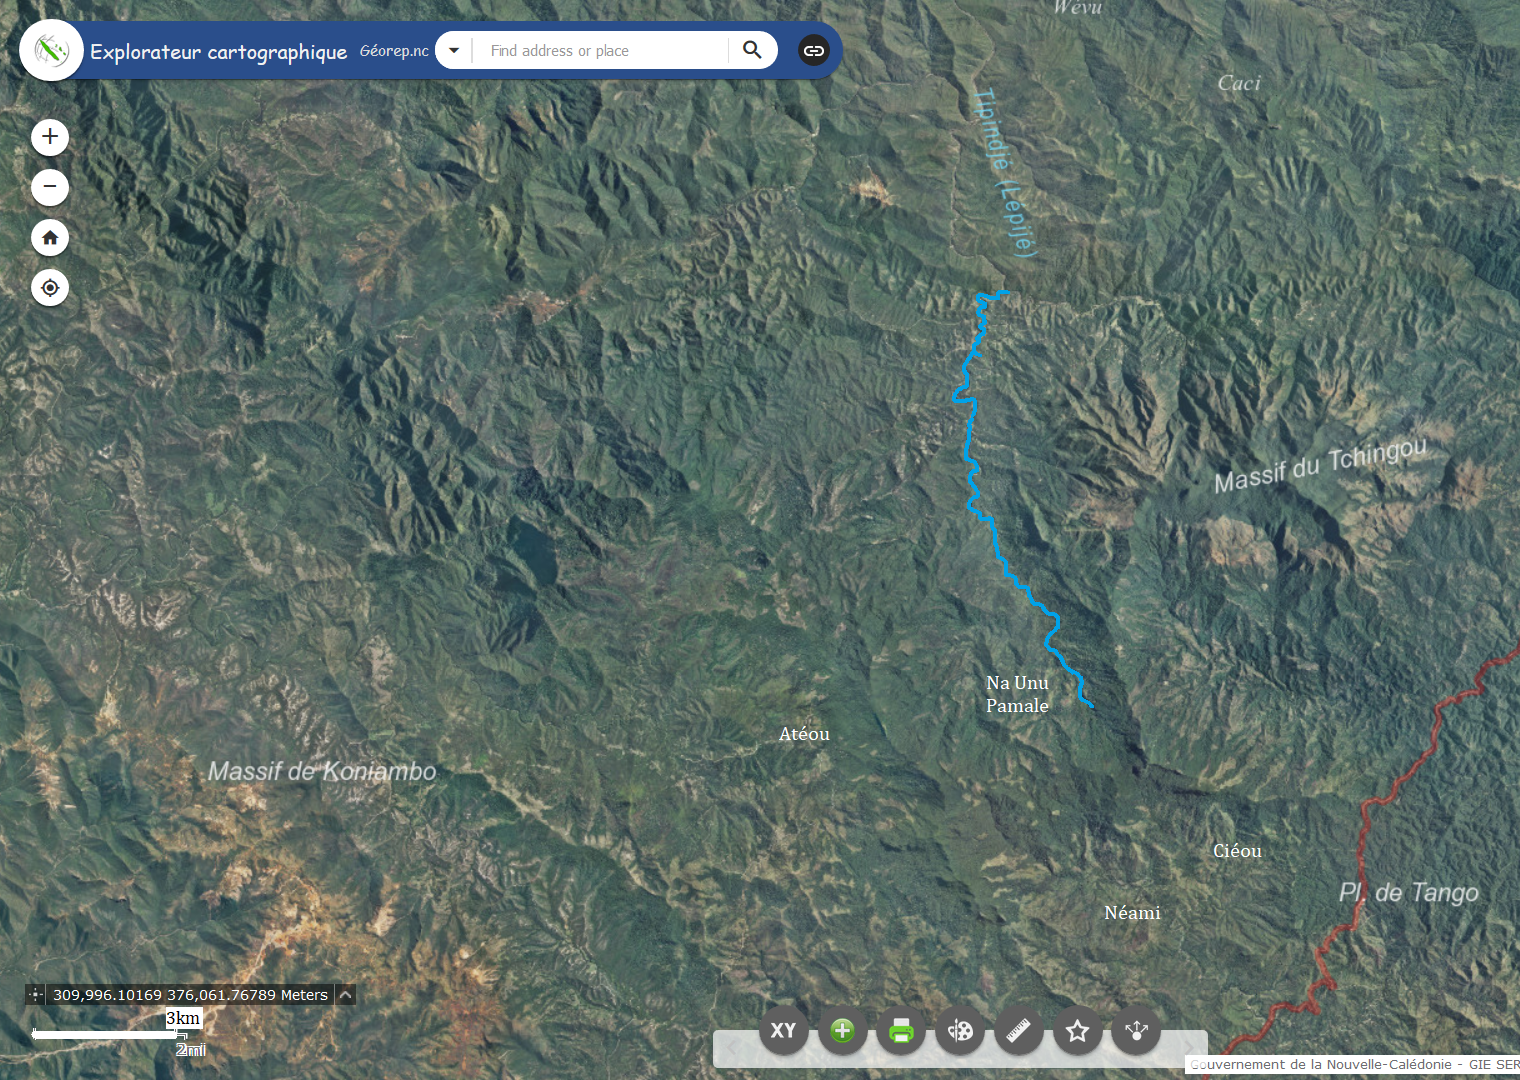
\includegraphics[width=\linewidth]{figures/ye_olde_mappe2}
	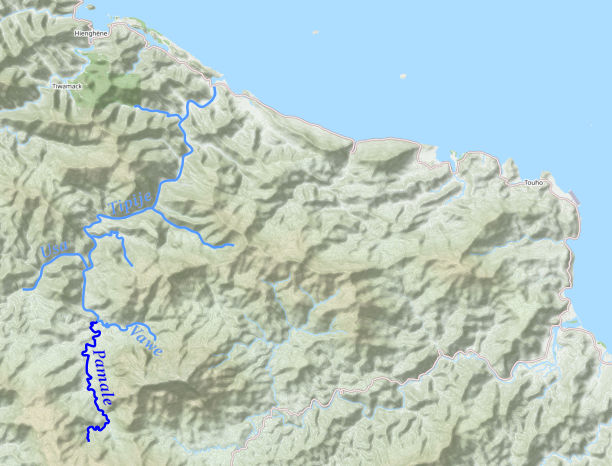
\includegraphics[width=\linewidth]{figures/pamale.pdf}
	\caption{Map of the Pamale river}
	\label{map:pamale}
\end{figure}

The Vawe, Pamale, and the upper Tipije valleys are said today to have been inhabited by Vamale speakers. Pamale is said to have been a great chieftaincy \parencite[59]{gohoup_guerre_2008}. The North of the island, roughly north of the Cèmuhî domain, was loosely structured into two alliances: \textit{Hoot} \qu{great tide} and \textit{Whaap} \qu{raven}, today eponymous of the customary area \textit{Hoot ma Whaap}. The Tipije valley was \textit{Hoot} but the later refuges of Pamale people, Wanas/Wanaa, Temala and Tiéta, were \textit{Whaap} \parencite[6]{guiart_lorganisation_1954}, so a cautious assumption may be made that Pamale refugees followed old paths of alliance. See \Cref{map:clans} for a visual representation of Guiart's analysis. %On the other hand, the Pamale refuge \textit{We Hava} is in the middle of the \textit{Hoot}-aligned Tipije and used to be ruled by Pamale's traditional ally\footnote{\parencite[272]{guiart_evenements_1970}} Kafeyat Batepoanwhane/Batpawan/Cidopwaan \qu{Nametaker Erect-Phallus}, who could retreat to Ouiou (\textit{Wévu} on map \ref{map:history}), which is relatively far upstream and quite likely \textit{Hoot}. 

\begin{figure}
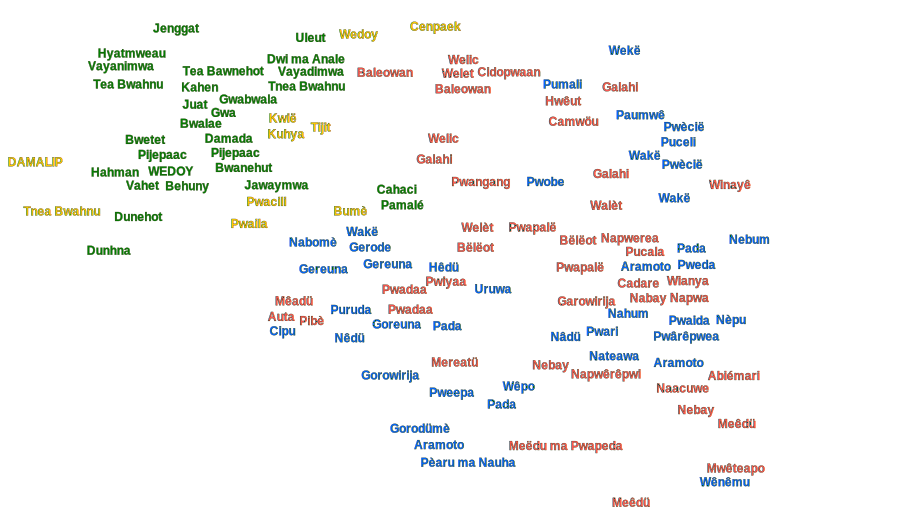
\includegraphics[width=\linewidth]{figures/clans_blur.pdf}
\caption{Selection of precolonial clans adapted from Guiart's 1979 map \textit{Clans autochtones: Situation pré-coloniale}, %with black underlines for yam masters, red for sun/rain
%masters, purple for taro masters, and dark brown for thunder masters,
green highlights for Hoot and yellow for Hwaap lineages, red for Bai and blue for Dui. \parencite[71]{guiart_clans_1981}}
\label{map:clans}
\end{figure}

The local distribution of languages before the 19\textsuperscript{th} century is difficult to estimate. However, around the turn of the last century, the land between the Cigu mountains and Koné, south of the Hienghène and at least up until Wan Kuut is likely to have been speaking varieties of Hmwaeke/Vamale. Clans speaking it almost certainly formed minority speaker populations in the allied valleys of Wanaa(s) (Ouanache), Thexhwaade (Tiouandé), We Hava, Pwey (Poyes), and on the other side of the mountains in Temala, Ceta (Tiéta), and Koogo (now deserted), as frequent exchanges were maintained with these villages, and this is where the refugees went (see \Cref{map:fugitives}). The chiefs of Wanaa and We Hava spoke Vamale \parencite[20]{leenhardt_evenements_1978a}.
\begin{figure}
% 	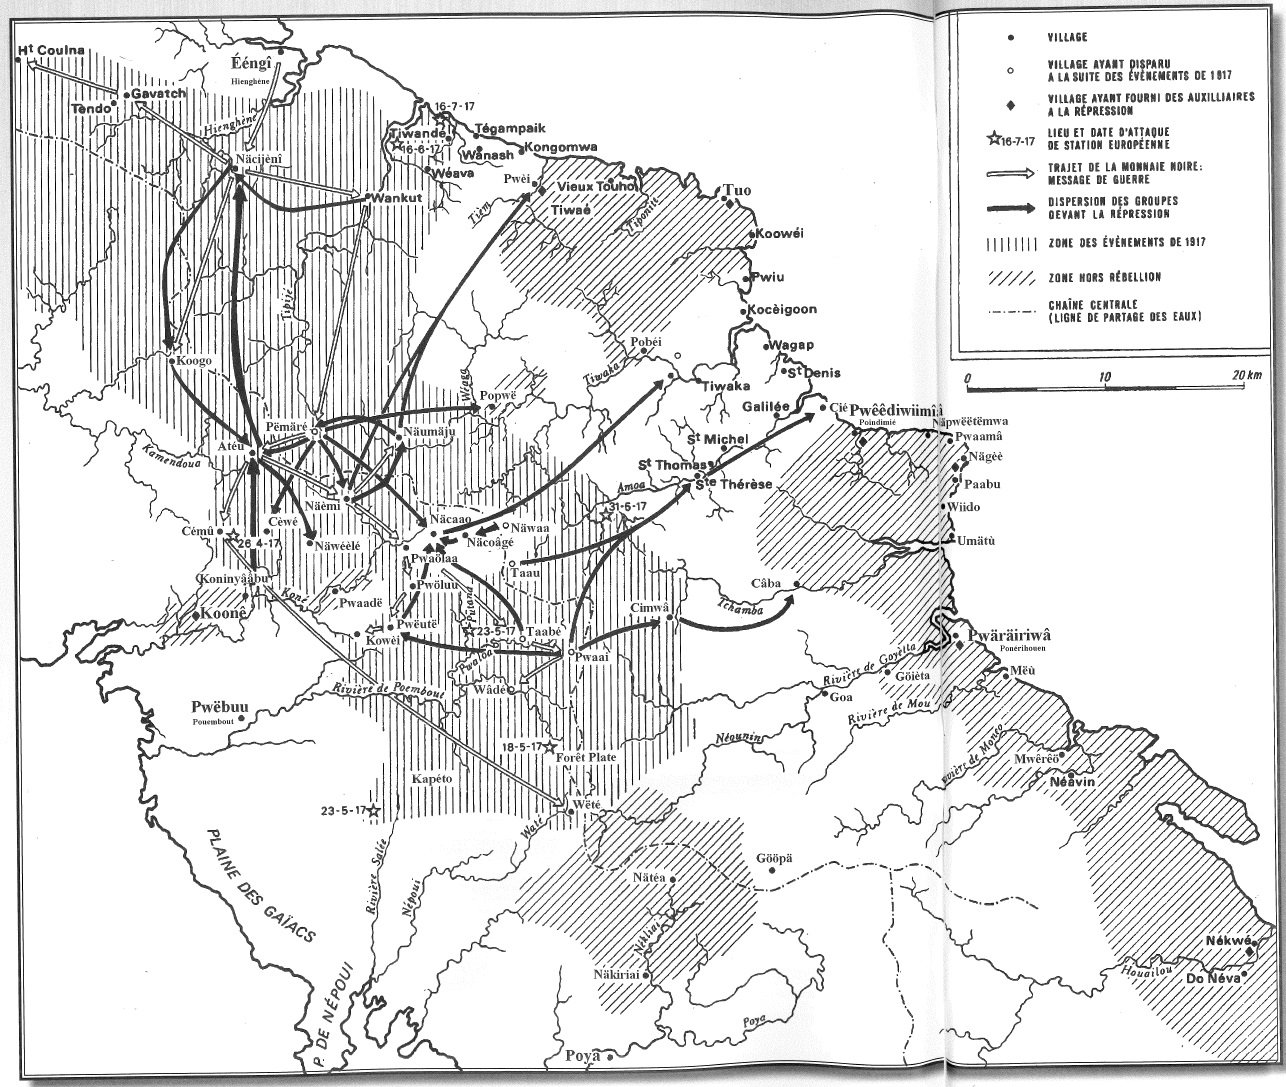
\includegraphics[width=\linewidth]{figures/prov_map_fug}
	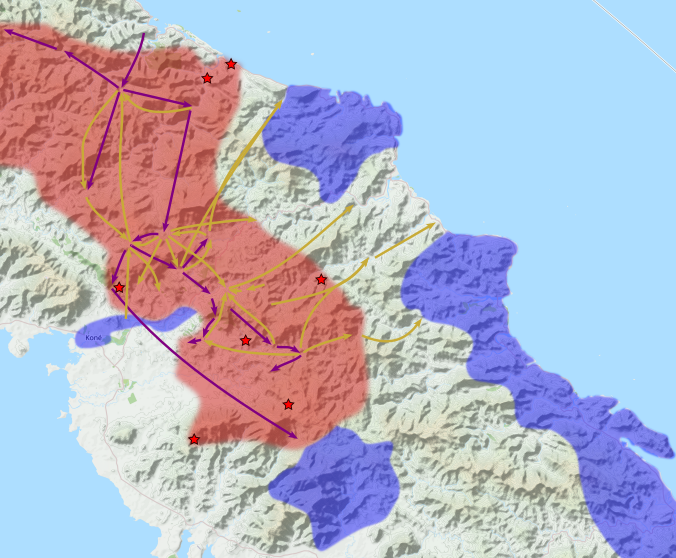
\includegraphics[width=\linewidth]{figures/refugees.pdf}
	\caption{Main movements of refugees following 1917 \parencite[7]{bensa_1917_2008}. Many movements leave Pamale (``Pëmärë").}
	\label{map:fugitives}
\end{figure}

%\begin{figure}
%	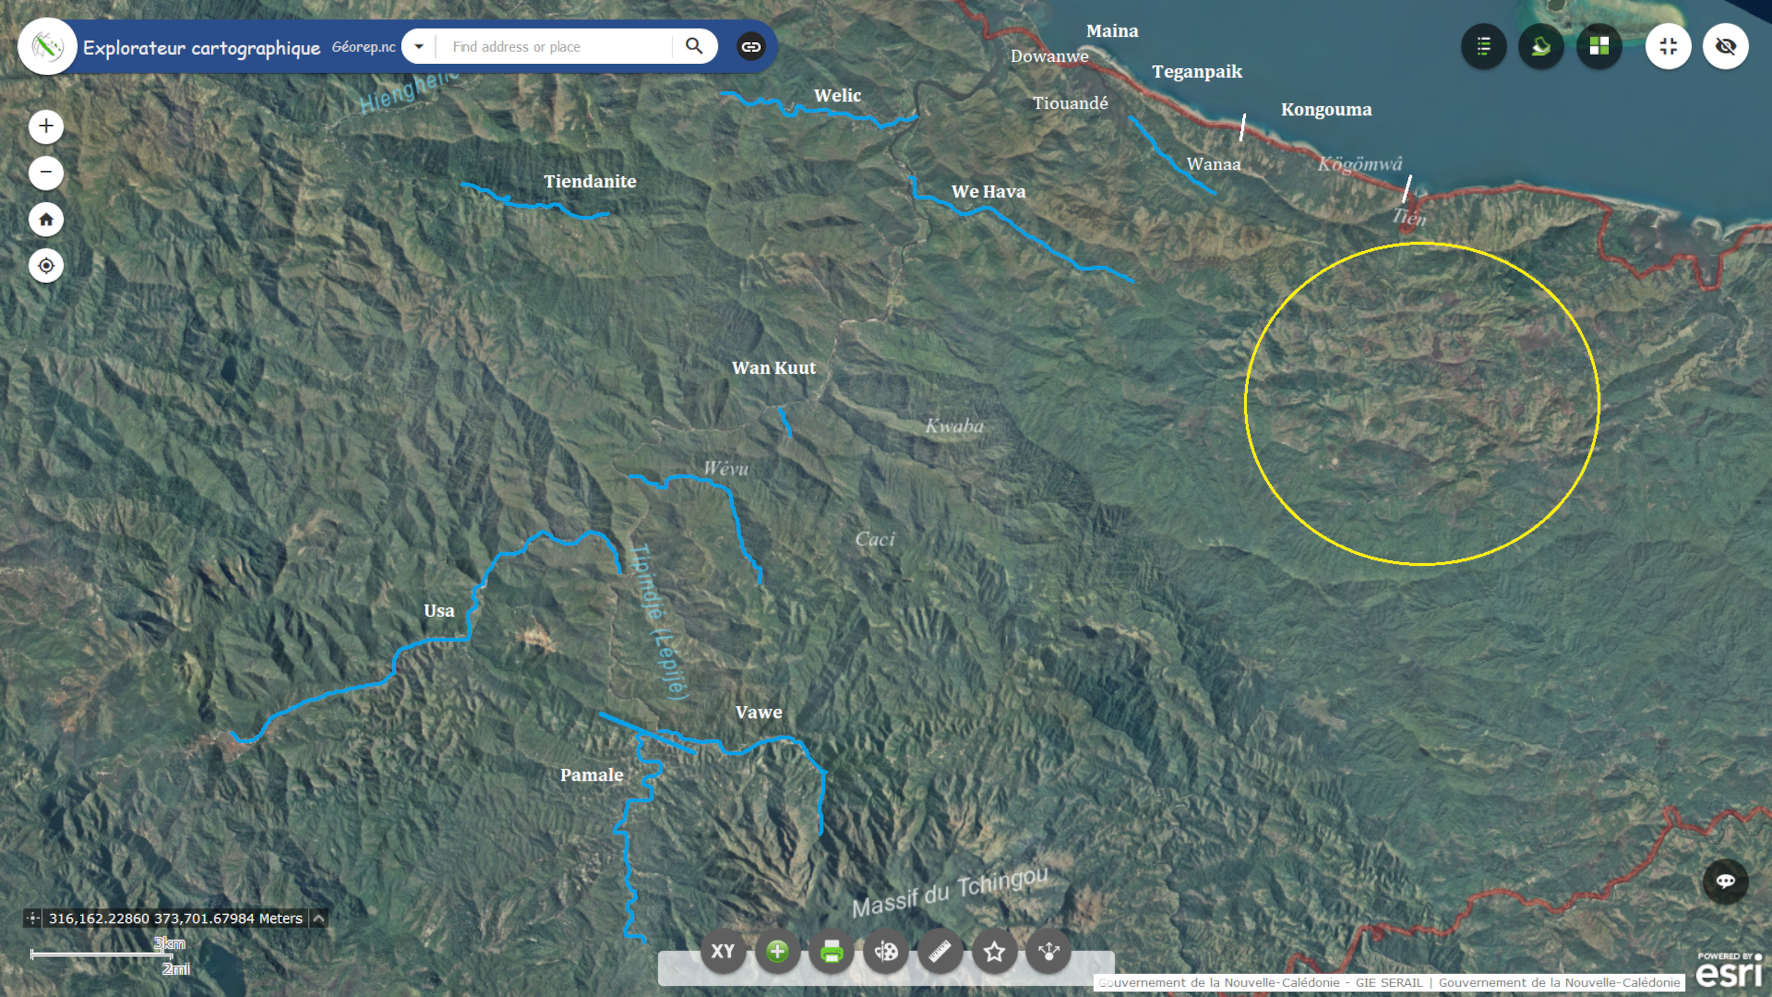
\includegraphics[width=\linewidth]{figures/ye_olde_mappe_politics}
%		\caption{Map of the area with main valleys. Poyes is circled in yellow. \cite{gouvenementdelanouvelle-caledonie_explorateur_2019}}
%	\label{map:history}
%\end{figure}

\section{The 1917 War}
On May 10\textsuperscript{th} 1901, a peace meeting took place in Pamale (\textit{Paix de Pamalé}). At the time, the area was not yet directly concerned by land spoliations or missions, though oral accounts speak of Pamale as a refuge for people driven from their lands \parencite[368, 369]{bensa_sanglots_2015}. The parties discussed the ``Affair of Poyes", a conflict between war chief Amane of Poyes and chief Hippolyte of Touho. Whatever the real reason was -- a woman, capitation tax, cooperation with Europeans, or land -- the two reconciled. \is{Affair of Poyes}

On the one side was Amane, a powerful war chief in the Cèmuhî-speaking village Poyes, who claimed land all the way till Paola on the west coast, according to a police report \parencite[24]{leenhardt_figures_1978}. He was a brother of Bwiyang, chief of Poyes. According to Amane himself, he had been promised since birth a woman whom Hippolyte of Touho took for himself. Amane wanted her back. Another explanation is the difference in stance towards Europeans. Hippolyte was Catholic and in close cooperation with European missionaries. Due to his exposed situation on the coast, his father Napoléon had already been in contact with Europeans, whereas Poyes remained relatively independent \parencite[21]{leenhardt_evenements_1978a}. According to (Protestant) Leenhardt, Hippolyte ruling over a militarily weak tribe \parencite[28]{leenhardt_figures_1978} was manipulated by the local Catholic missionaries, the peace meeting was an overreaction and the Poyes had not even attacked yet. It may also have concerned the capitation tax \parencites[23]{leenhardt_figures_1978}[13]{philcat_revolte_1989}, which Amane refused to pay, whereas Hippolyte cooperated with the occupier. In any case, Amane met with his adversary, and Governor Paul Feillet, the missionary Maurice Leenhardt, as well as Kanak dignitaries from as far away as Houailou, for a peace palabre \textcite[24]{leenhardt_figures_1978}. The two reconciled. 
After the peace meeting, the \qu{Thunder of Poyes} Amane held several reunions in Pamale. 

Possibly in response to this subversive behavior \parencite[289]{saussol_lheritage_1979}, or because Pamale was a safe haven for refugees, the Pamale lands' reservation status was revoked by the government by the (unpublished) \textit{arrêté} n°775 on June 30\textsuperscript{th} 1903 \parencite[282]{guiart_evenements_1970}, enacted on July 30\textsuperscript{th} 1904 \parencites[92]{guiart_laire_1992}[22]{philcat_revolte_1989}. %\todo{check}

The reservation status had been Pamale's only protection from state-sanc\-tioned spoliations \parencite[3]{demmer_nationalisme_2003}, and the land was bought by the Belgian cattle rancher Charles Metzdorf. He founded a cattle ``station", a ranch, at Pamale \parencite[273]{guiart_evenements_1970}. The same year, possibly to avoid conflict with the population, Metzdorf's manager brought in \textit{gendarmes} who burned the houses of the Pamale, as well as the houses and the Protestant temples in Pije-speaking Pupay (Puepaek) and in Paada, and the village of Pwekea Kalemumak (upper Voh valley, probably Haveke-speaking) \parencite[266]{guiart_evenements_1970}. This act of war may have targeted clans who were allied to Pamale families and their neighbors, and who could have taken in refugees. Governor Feillet claims his group arrived on Charles Metzdorf's cattle-station in Pamale on the 10\textsuperscript{th} of May 1901 and slept in the recently abandoned cattle station in Vawe\is{Metzdorf, Charles} \parencite[26]{leenhardt_figures_1978}, both of which can only have existed legally 3 years later, after Pamale was erased from the map with fire and guns, as mentioned above \parencite[27]{leenhardt_figures_1978}. Governor Feillet cannot have confused the dates because he left for France on October 18\textsuperscript{th} 1902 and died in Montpellier September 2\textsuperscript{nd} 1903 \parencite[29]{leenhardt_figures_1978}. Whether Metzdorf came earlier than officially claimed and then had the reservation revoked in order to avoid neighborly conflicts with the dispossessed former inhabitants could not be reconstructed by the author. Metzdorf would later leave the area to be succeeded by the Ouaco mining company. It, too, left by the early 1930s \parencite[266]{guiart_evenements_1970}. The land is now in customary hands and used as hunting grounds by the villages Néami and Noéli.

%\begin{figure}
	%\centering
%	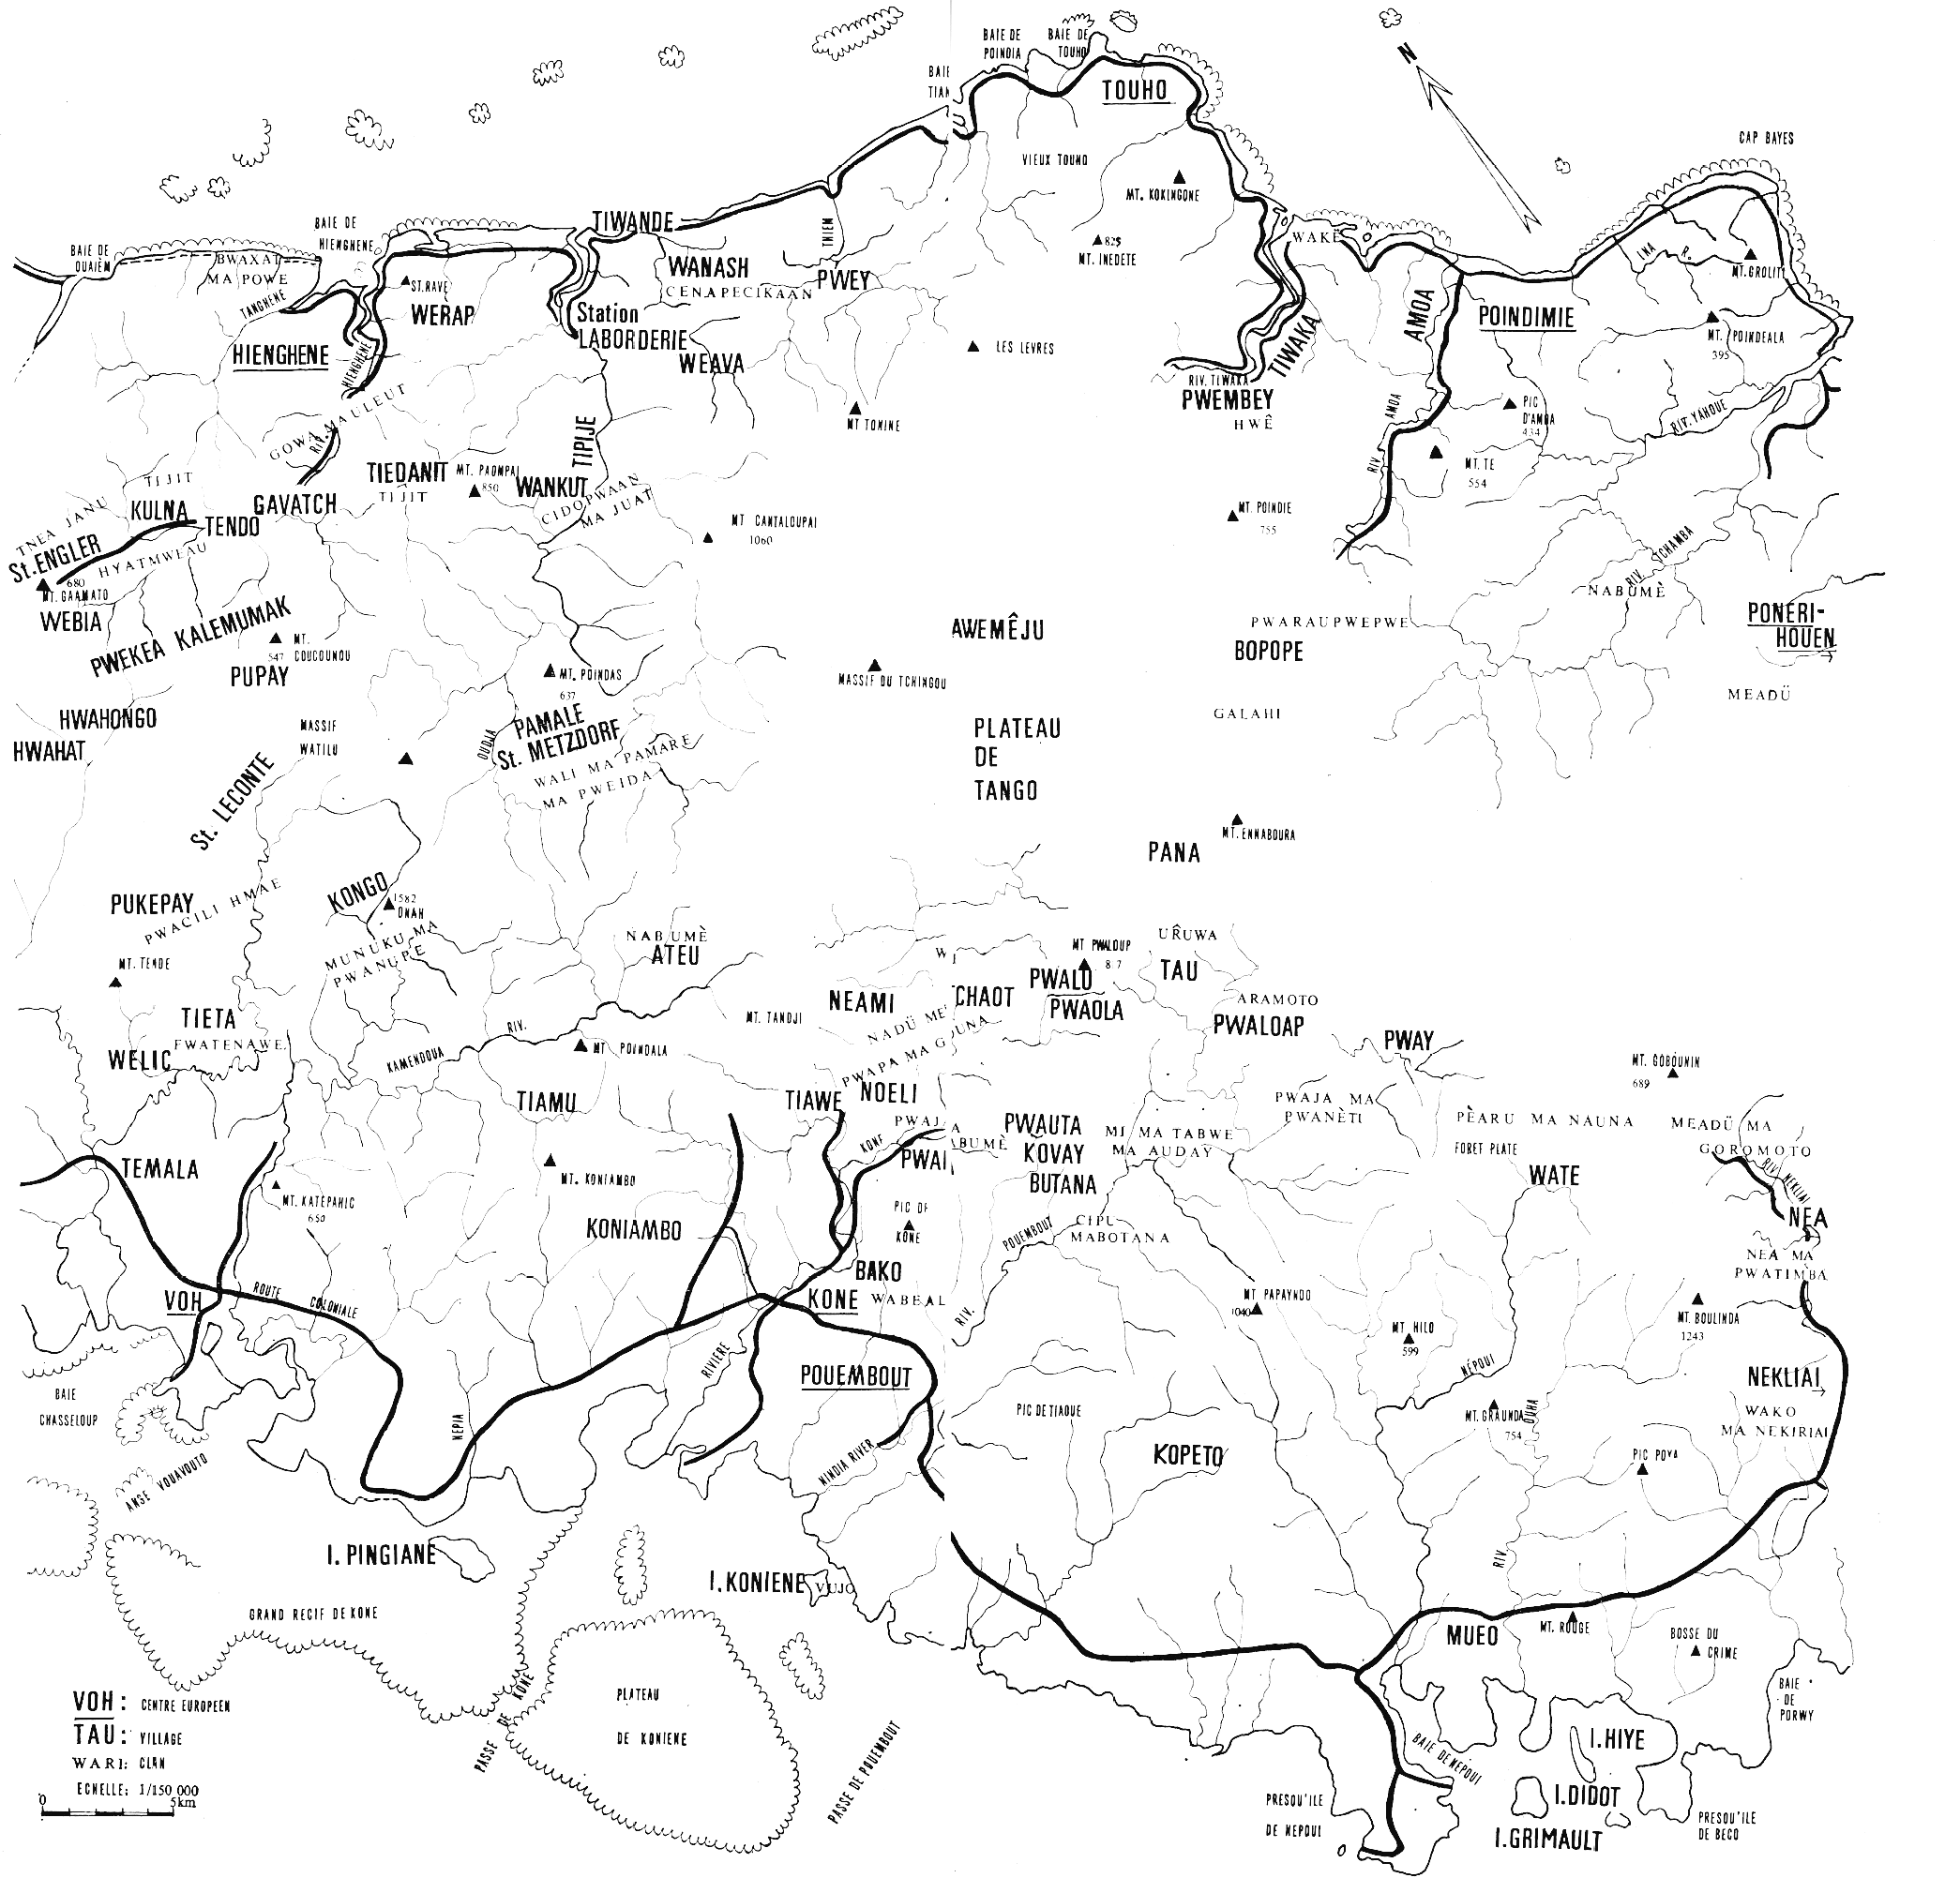
\includegraphics[width=\linewidth]{figures/pamale_guiart}
%	\caption{A map of main Kanak villages around 1913 \parencite[269]{guiart_evenements_1970}}
%	\label{fig:Guiart}
%\end{figure}

As a reaction to the destruction of their houses, the Pamale tribe,\footnote{Since a decentral spatial organisation was described for Pamale in 1857, I use the same term as my sources here instead of ``village", which is more appropriate for the current situation.} which had\is{Tipije War} moved north, hosted war \textit{pilous}\footnote{A Kanak word for \qu{dance}, \textit{vila} in Vamale, for festive meetings and palabres.} in 1913 \parencite[266]{guiart_evenements_1970}. This took place in a simmering martial context, and several attacks from various tribes on European stations erupted all over the area in the years after. A book dedicated to the topic is \citetitle{bensa_sanglots_2015} (\citeauthor{bensa_sanglots_2015}, 2015). 

The Bwaarhat clan, great chiefs of the Fwâi-speaking Hienghène coast, had been in conflict with the European forces since the 19\textsuperscript{th} century, and several generations of chiefs had been sent to exile in Tahiti \parencite[102]{clifford_person_1982}. When Bwaarhat sent the black war money up the Tipije, its great chief Kafeyat Cidopwaan sent it further up to Pamale.\footnote{He, too, is a controversial figure. Muckle expands on his changing reputation with the colonial government \parencite[139--141]{muckle_troublesome_2010}.}

The Tipije war of 1917 broke out after long discussions between the chieftaincies. Whether Pamale's chief Athea Sergent Mërëatu actually agreed to participate in the fighting or not is unclear, %depends on whom one asks nowadays
but does not seem to have played a crucial role. He was not a chief of an existing settlement anymore % (but allied tribes participated in the raids 
\parencite[277]{guiart_evenements_1970}. Warriors from Pamale were among those who slaughtered the Grassin family, the settler Papin and the Tahitian soldier Elizera in We Hava on June 16\textsuperscript{th} 1917 \parencite[24]{boubin-boyer_nouvelle-caledonie_2015}. They were also part of the war party from whom the settler Ragot in Wanaa was saved either by Leenhardt (according to his descendant, \citealt[20]{leenhardt_evenements_1978a}) or defended by the locals (according to Ragot's descendants). 
%\begin{quotation}Le 16 juin, à Oué Hava, une vallée proche de Hienghène, le colon Henri Grassin, sa femme Clémence, leur domestique javanais, Sastiviredjo et leur voisin Ludovic Papin sont massacrés par les hommes de Noël Kaveat et une quarantaine de guerriers de Pamalé, de Ouenkout et d’Atéou. Le cadavre d’Henri Grassin a été éviscéré.\end{quotation} (\parencite[24]{boubin-boyer_nouvelle-caledonie_2015}:24)
In total, 8 settlers were killed in the area. As a result, almost every village, involved or not, was burned down between Koné and Poyes. Over a dozen villages in the Tipije valley and its tributaries have disappeared, including the ones to which Pamale residents had fled after their valley's destruction in 1904. While this account focuses on Vamale, the majority of the villages concerned were Pije-speaking, a language which is now even more endangered than Vamale.\is{Tipije War}


\begin{figure}
	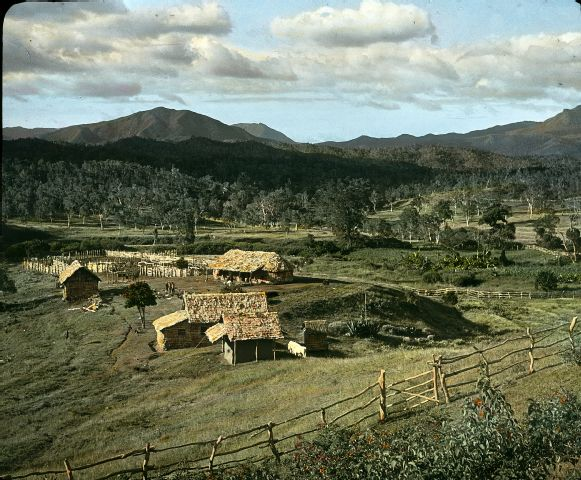
\includegraphics[width=.8\linewidth]{figures/metzdorf}
	\label{fig:metzdorf}
	\caption{Metzdorf's cattle-ranching station. CC-BY-SA Heim, \parencite{heim_farm_1921}}
\end{figure}


Philippe Dego Gohoupe (``Hao Cakeo")'s account from the 11\textsuperscript{th} November 2016 claims that Vamale speakers came from Mt. Pamale further southwest in the mountain range, and at some point moved to the valley of Tipije, whence they were chased in 1917. This is confirmed by late Galé Kalen's account from the 6\textsuperscript{th} September 2017, as well as \textcite{bensa_political_1997} and \textcite{leenhardt_figures_1978}, among others. A resettlement of the Pamale valley is unlikely in the near future, as it is considered cursed and the traditional ownership is far from clear. Some families fled to Tiendanite (confirmed by Agnès Wathea, 29.11.2017), while others chose to follow the Tipije river down to its tributary We Hava and the Pije-named coastal villages Téganpaïk, Wanaa and Tiouandé. This would explain not only the dispersion of the community, but also the languages with which they are in contact: Pije, Nemi, and Fwâi\footnote{Tiendanite and We Hava send their children to school in Fwâi-speaking Hienghène.} for Tiendanite and We Hava, Pije and Cèmuhî for the coastal villages.

The Usa variety is nowadays spoken in Tiendanite. Politically, Tiendanite is chief Goa's domain, a rival of chief Bwaarhat, whereas in 1917, Wan Kuut's chief Kavéat was an ally of both Bwaarhat and Pamale's Athea Sergent. Usa speaker Agnès Wathea mentioned that her father's clan, from Usa, was welcomed to Tiendanite by its chief, though Usa was under Athea's control, and thus not a village allied to Tiendanite. Furthermore, Vamale speakers are likely to have been on the coast prior to the war. Although the coast was disturbed by European presence, Vamale-speaking chiefs were already well in place in We Hava and Wanas by 1917 \parencite[20]{leenhardt_evenements_1978a}. Overall, this suggests a speaker mobility on an individual and family level that was relatively unimpressed by chiefs and higher politics, and followed personal alliances. This is supported by Bensa's map in \Cref{map:clan_movements}, which shows a visual representation of three oral histories, mostly pre-colonial. Regardless of this free individual networking, most family histories are tainted by the war.%, which can affect current projects, e.g. regarding research or tourist infrastructure. 

\begin{figure}[t]
% 	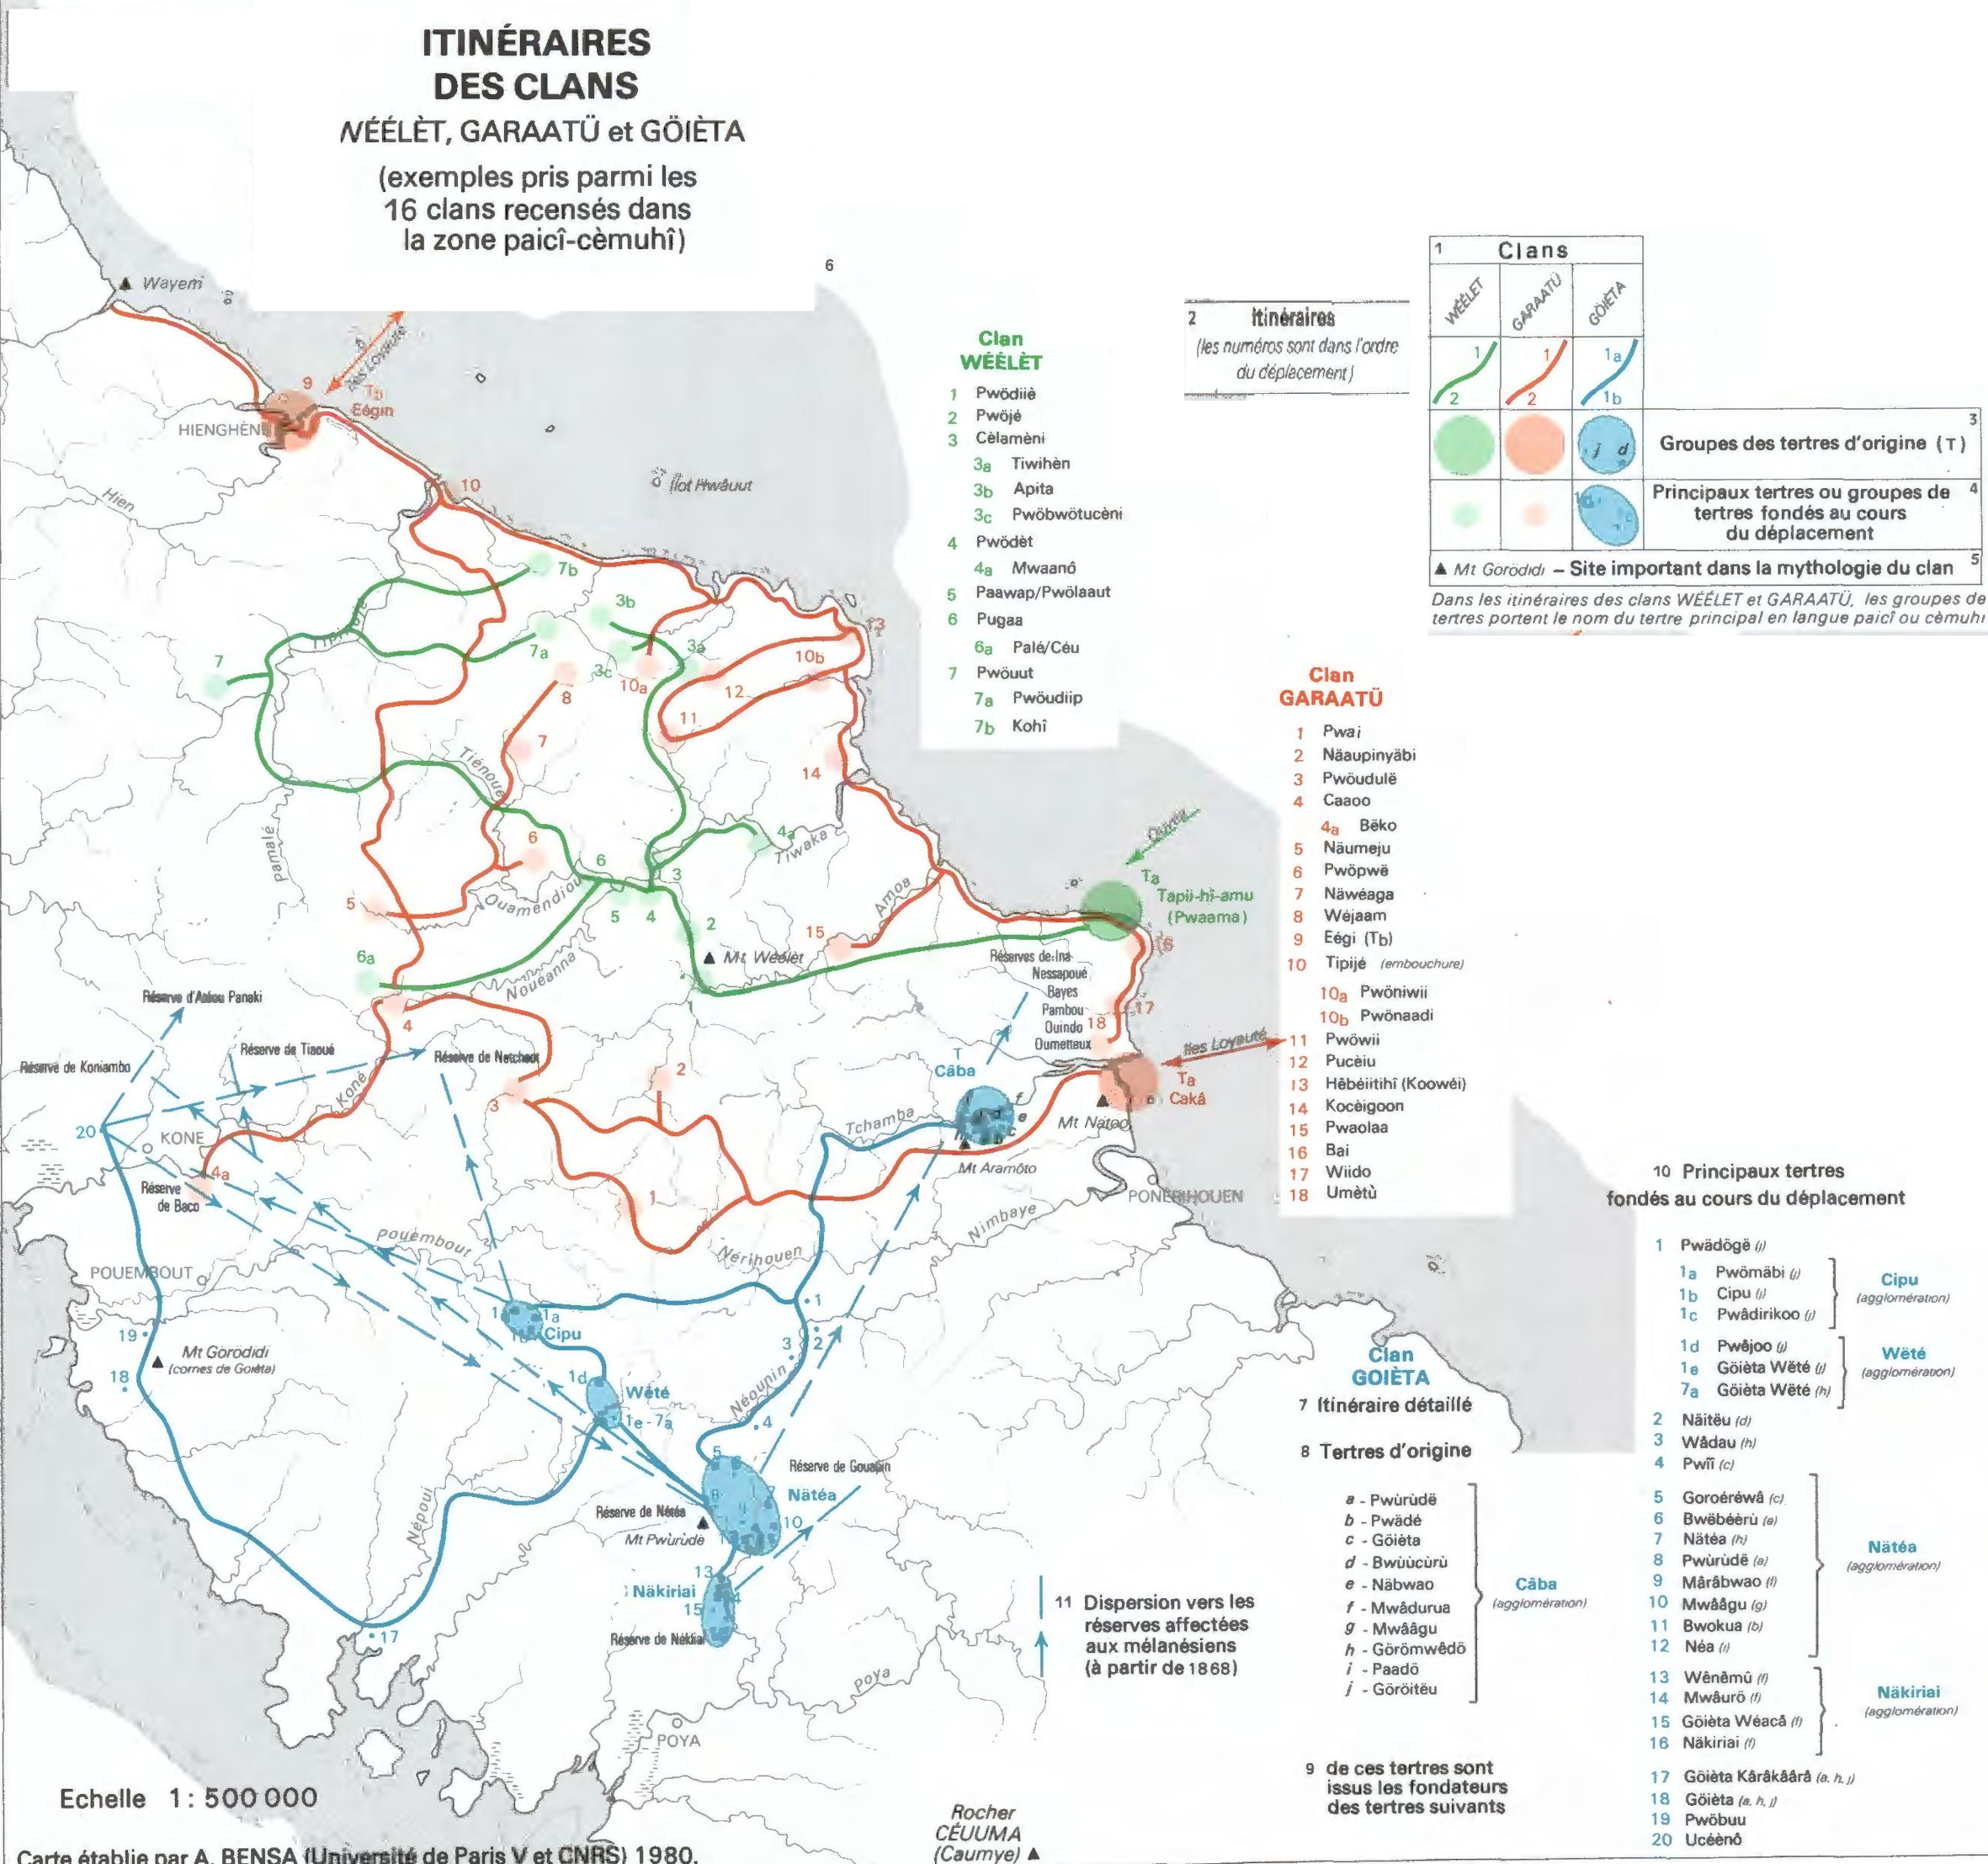
\includegraphics[width=\linewidth]{figures/clan-movements}
	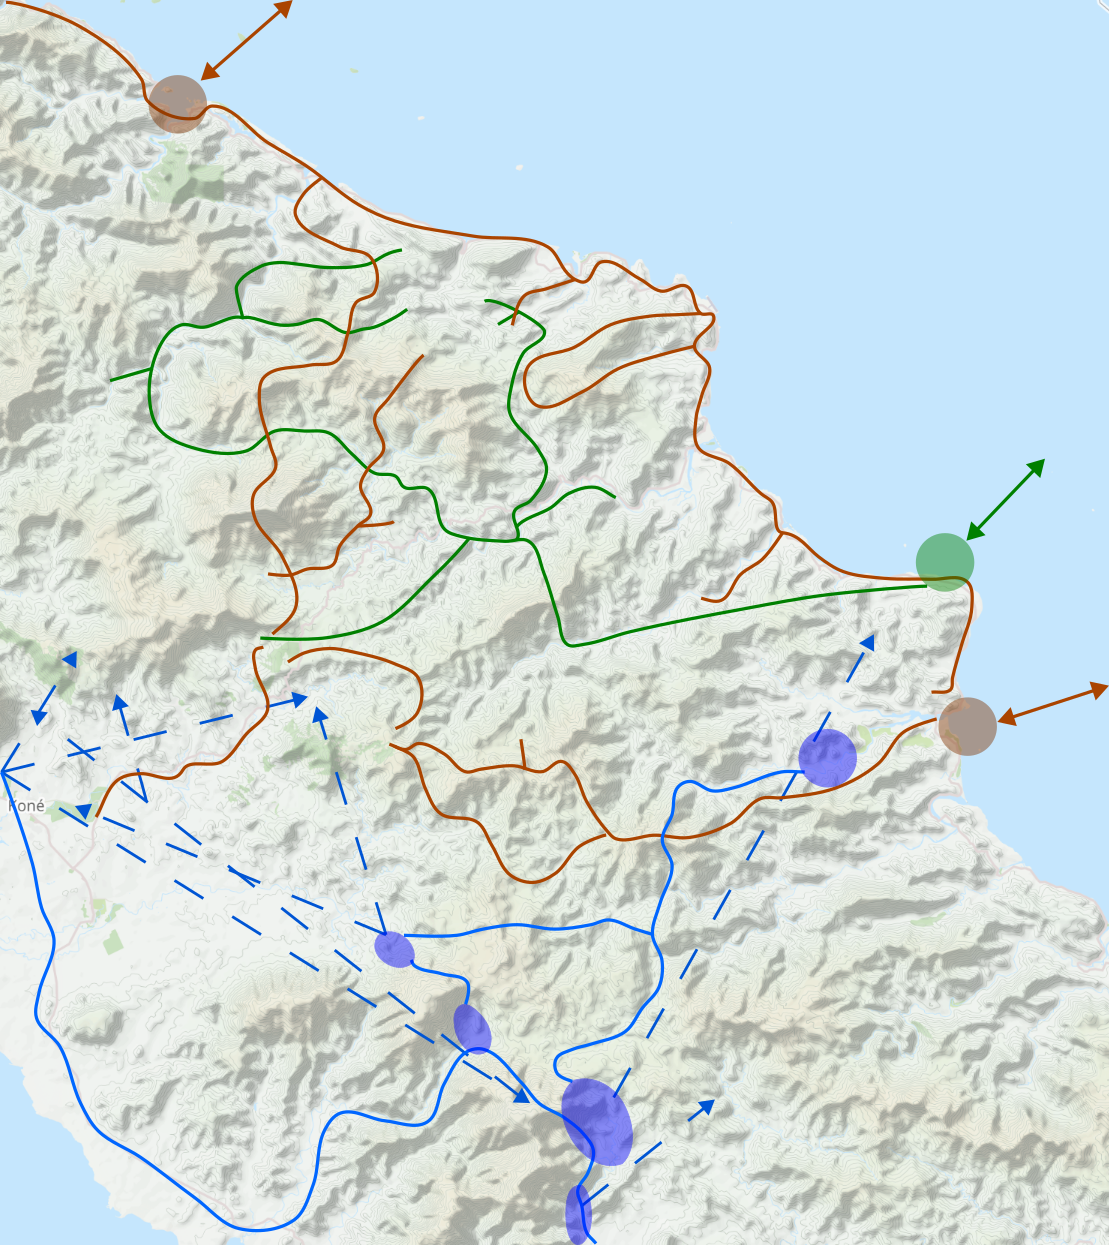
\includegraphics[width=.8\linewidth]{figures/clans.pdf}
	\caption{Map showing some clans' migrations in the Touho-Hienghène area, following \cite[71]{guiart_clans_1981}}
	\label{map:clan_movements}
\end{figure} 


\section{French policy and decline of the language}
\label{ssec:Frenchpolicy}
After the war, contact with the French and their language was sporadic until the 1950s. The colonial government locked Kanaks of diverse origins into reservations, hoping that their catastrophic demographic decline from perhaps 400,000{\interfootnotelinepenalty=10000\footnote{``To our knowledge, the only person to have proposed a density model for Grande Terre was the geographer J. P. Doumenge, who believed in a low population of about 65,000 people at contact. Nevertheless, he proposed a density of ``130 to 145 inhabitants per square kilometer of used horticultural surface'' (\citealt[463]{doumenge_terroir_1982}, original text in French). Reducing his figures by half (i.e., seventy p/km\textsuperscript{2}) to account for the vague status of the phrase \qu*{used horticultural surfaces}, and again using only one-third of the surface of the island, we would arrive at 400,000 people." \parencite[316]{sand_what_2007}}} people before contact \parencite[316]{sand_what_2007} to just about 27,000 in the early 1920s \parencite[309]{sand_what_2007} would in time lead to a total disappearance in contact with a ``superior race" \parencites[289]{stern_colonies_1943}[2]{salaun_francophonie_2005}. French colonial language policy was not very invasive and concentrated on prohibiting the use of indigenous languages in public\footnote{The ``public" being defined by the presence of settlers.} \parencite[2]{salaun_francophonie_2005}. However, most Kanaks were confined to reservations \parencite[3]{demmer_nationalisme_2003} in which the only outsiders were missionaries and \textit{gendarmes}, so even that policy did not affect many people. %hence little influence

The event truly leading to speaker decline was schooling, which only began on any scale to speak of in the 1950s.\footnote{Note that Leendhardt counted only around 50 speakers in the 1940s, but schooling prevented a subsequent language transmission, and therefore a quicker recovery.} Before that, Kanaks were not citizens,\footnote{The \textit{Code de l'Indigénat} specifying this was abolished in 1946, but this was not noticeably implemented until 1952.} and the only schooling was privately done by the churches. Most elders in the villages do not enjoy speaking French and are multilingual in Kanak languages. Until the 1980s, the Vamale-speaking area was untouched by public schooling. Most children went to the Protestant private school in Tiouandé (\textit{Fédération de l'enseignement libre protestant}, F.E.L.P., closed in the 1980s) or to Catholic institutions like the one in Tuo Mission. Nowadays, all children go to the public schools in Hienghène (for Oué Hava) and Touho (for Tiouandé and Téganpaik), where the dominant Kanak languages are Fwâi and Cèmuhî respectively. TV, radio, the spread of smartphones and the advent of mobile internet in early 2019 have added to language contact. 

%Having touched upon the history of Vamale as known by European sources, and complemented by Kanak oral sources, the present situation is described below, first in terms of human geography.

% \section{Modern context}


